\documentclass[11pt,reqno,final]{amsart}

\pdfcompresslevel=0
\pdfobjcompresslevel=0

\usepackage[dvipsnames]{xcolor}% adds colors
\usepackage{amsmath, amsthm}% {amsfonts, amssymb}

% New Characters
\usepackage[latin1]{inputenc}%
\usepackage[T1]{fontenc}

\usepackage{MnSymbol}
\usepackage[normalem]{ulem}% underlining

\usepackage[theoremfont, largesc]{newpxtext} % different text,math font
\usepackage{newpxmath}

\makeatletter
\DeclareMathRadical{\sqrtsign}{symbols}{112}{largesymbols}{112}
\let\sqrt=\undefined
\DeclareRobustCommand\sqrt{\@ifnextchar[\@sqrt{\mathpalette\@x@sqrt}]}
\def\@x@sqrt#1#2{%
 \setbox\z@\hbox{$\m@th#1\sqrtsign{\mkern1mu #2}$}
 \mkern3mu\box\z@}
\makeatother




% Page Typesetting
\usepackage[final]{microtype}
\usepackage{relsize}
\usepackage[margin=1in]{geometry}
\usepackage{framed}
\usepackage{tikz}

\usepackage{hyperref}
\hypersetup{
  final,
  pdftitle={Math 135 - Limits},
  pdfauthor={Bonventre}, 
  linktoc=page,
  pagebackref,
  colorlinks=true,
  citecolor=PineGreen,
  linkcolor=PineGreen,
  linkbordercolor=PineGreen,
}


% Internal References

\usepackage[inline,shortlabels]{enumitem}

\numberwithin{equation}{section} 
\numberwithin{figure}{section}

\usepackage[nameinlink,capitalise,noabbrev]{cleveref}

\crefname{equation}{}{} % get \cref to behave as \eqref

% \theoremstyle{plain} % bold name, italic text
\newtheorem{theorem}[equation]{Theorem}%
\newtheorem*{theorem*}{Theorem}%
\newtheorem{lemma}[equation]{Lemma}%
\newtheorem{proposition}[equation]{Proposition}%
\newtheorem{corollary}[equation]{Corollary}%
\newtheorem{conjecture}[equation]{Conjecture}%
\newtheorem*{conjecture*}{Conjecture}%
\newtheorem{claim}[equation]{Claim}%
\newtheorem{question}{Question}

\theoremstyle{definition} % bold name, plain text
\newtheorem{definition}[equation]{Definition}%
\newtheorem*{definition*}{Definition}%
\newtheorem{example}[equation]{Example}%
\newtheorem*{example*}{Example}%
\newtheorem{remark}[equation]{Remark}%
\newtheorem{notation}[equation]{Notation}%
\newtheorem{convention}[equation]{Convention}%
\newtheorem{assumption}[equation]{Assumption}%
\newtheorem{exercise}[question]{Exercise}

% ---------- macros
\newcommand{\set}[1]{\left\{#1\right\}}%
\newcommand{\sets}[2]{\left\{ #1 \;|\; #2\right\}}%
\newcommand{\longto}{\longrightarrow}%
\newcommand{\into}{\hookrightarrow}%
\newcommand{\onto}{\twoheadrightarrow}%

\usepackage{harpoon}
\newcommand{\vect}[1]{\text{\overrightharp{\ensuremath{#1}}}}

\newcommand{\del}{\partial}%

\newcommand{\ki}{\chi}
\newcommand{\ksi}{\xi}
\newcommand{\Ksi}{\Xi}

% %%%%%%%%%%%%%%%%%%%%%%%%%%%%%%%%%%%%%%%%%%%%%%%%%%%%%%%%%%%%%%%%%%%%%%%%%%%%%%%%%%%%%%%%%%%%%%%%%%%%

\begin{document}

\begin{center}
        \textbf{\Large Math 135, Calculus 1, Fall 2020}\\[10pt]
        {\large 09-16: Limits, Velocity, and Tangent Lines}
\end{center}

\thispagestyle{empty}

\renewcommand{\thesection}{\Alph{section}}

\section{Velocity}

Calculus is a set of tools to analyze functions.
Sir Isaac Newton, one of the founders, was motivated to invent the subject in order to verify Kepler's law of planetary motion.
In particular, this required an understanding of the mechanics of an objects \textbf{velocity}.

\begin{framed}
        If $s(t)$ describes the position of an object at time $t$,
        the \textbf{average velocity} over some time interval $[t_1, t_2]$ is given by the ratio of the change in position to the change in time:
        \[
                \text{average velocity} \quad = \quad \dfrac{\Delta s}{\Delta t} = \dfrac{\text{change in position}}{\text{change in time}} =  \dfrac{s(t_2) - s(t_1)}{t_2-t_1}
        \]
\end{framed}

\begin{exercise}
        A group of students are driving from Holy Cross to Boston for a day trip.
        \begin{enumerate}[(a)]
        \item It takes them 51 minutes to drive the 40 miles between Worcester and Boston.
                What was their average velocity on this leg of the trip?
                \vfill
        \item They hit traffic on the way back. If they left Boston at 5 pm and arrive back in Worcester at 7:30pm, what was their average velocity on their return trip?
                \vfill
        \end{enumerate}
\end{exercise}

\subsection{Geometric Interpretation}

Looking at the graph of the function $s(t)$, we see that $\dfrac{s(t_2) - s(t_1)}{t_2-t_1}$ also gives the \textbf{slope} of the
\textbf{secant line}, the line connecting the points on the graph of $s(t)$ at $t=t_1$ and $t=t_2$:
\begin{center}
        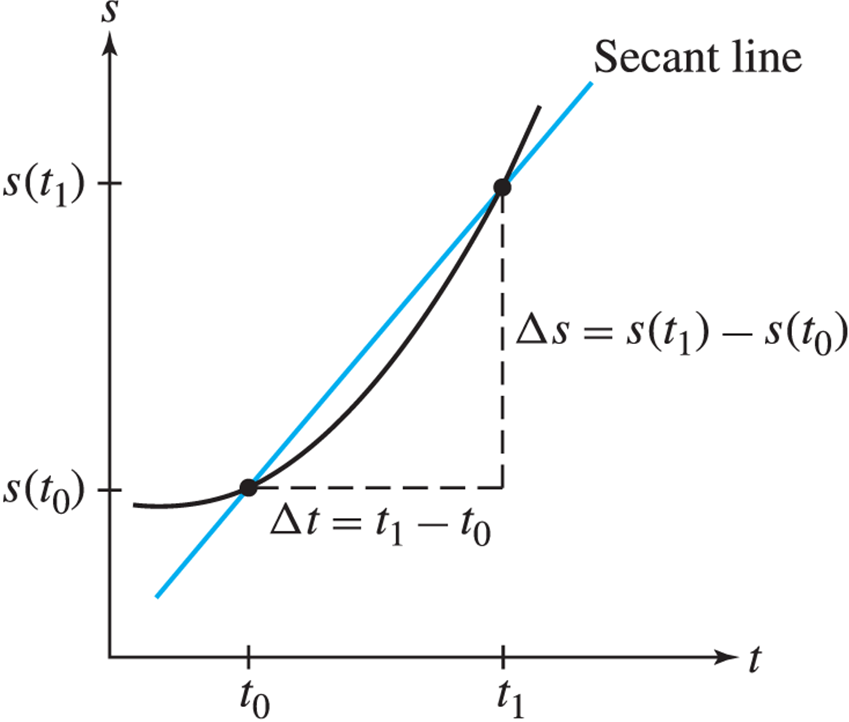
\includegraphics[width=3in]{09-16P-sec.png}
\end{center}

\newpage

\subsection{Instantaneous Velocity}

But Newton needed to know the \textbf{instantaneous velocity}, the speed at a particular moment in time, the ``speedometer reading''.
We can approximate this value by looking at the average velocity over smaller and smaller intervals:
\begin{exercise}
        \label{EX1}
        Suppose that $s(t) = t^2 + 4t+3$ describes the position of an object (in feet) at time $t$ (in seconds).
        Compute the average velocity over each of the following time intervals:
        \begin{enumerate}[(a)]
        \item $[1,2]$
                \vfill
        \item $[1,1.1]$
                \vfill
        \item $[0.99,1]$
                \vfill
        \item $[0.999, 1]$
                \vfill
        \item Based on these computations, what is the instantenous velocity at time $t = 1$?
                \vfill
        \end{enumerate}
\end{exercise}

\subsection{Geometric Interpretation}

As we look over smaller and small time intervals, the secant lines approach the \textbf{tangent line}, which abuts the graph at precisely one point:
Take a look at this Desmos demonstration: \url{https://www.desmos.com/calculator/8ubngtz3ei}.

Looking at the slopes of the secant lines, they \textbf{limit}, i.e. approach, a specific value: the slope of the tangent line.
\begin{framed}
        \begin{align*}
          \text{average velocity} &= \text{slope of secant line} = m_{sec}\\
          \text{instantaneous velocity} &= \text{slope of tangent line} = m_{tan}
        \end{align*}
\end{framed}

The slope of the tangent line is the \textbf{limit} of the slopes of the secant lines:
\[
        m_{tan} = \lim_{t_2 \to t_1} m_{sec}
\]
which we read as ``$m_{tan}$ is the limit of $m_{sec}$ as $t_2$ goes to $t_1$''.
This means:
\begin{itemize}
\item we are considering the quantity $m_{sec}$ as $t_2$ approaches $t_1$
\item the values of $m_{sec}$ appraoch some specific number
\item that specific number is in fact $m_{tan}$, the \textbf{limit}.
\end{itemize}

Limits are the technical heart of all of calculus.


\newpage

\section{Limits}

\begin{definition*}
        Given a function $f(x)$, we say that \textit{the limit of $f(x)$ as $x$ approaches $c$ is equal to the number $L$} if
        $|f(x)-L|$ can be made arbitrarily small by taking $x$ sufficiently close (but not equal) tto $c$.

        In this case, we write
        \[
                \lim_{x \to c}f(x) = L
        \]
        and say ``$f(x)$ approaches $L$ as $x$ goes to $c$''.
        \begin{center}
                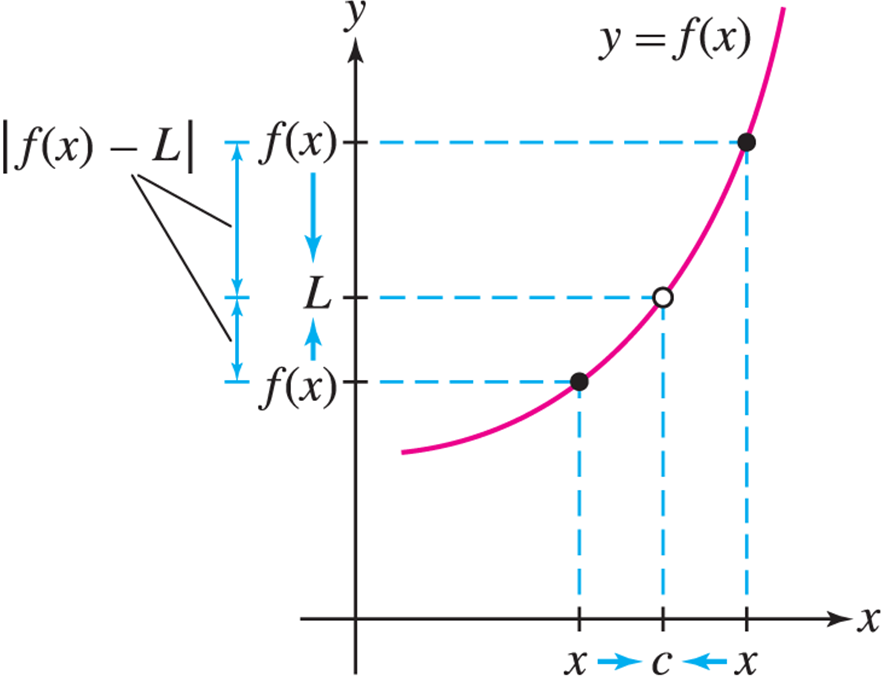
\includegraphics[width=2.5in]{09-16P-lim.png}
        \end{center}
\end{definition*}

\begin{example*}
        For \cref{EX1} we computed that
        \[
                \lim_{t \to 1}\dfrac{t^2+4t-5}{t-1} = 6.
        \]
        Note that, even though $\frac{t^2+4t-5}{t-1}$ is \textbf{not defined} at $t = 1$ (can't divide by 0), \textit{the limit still exists}.
        We only care about the value that the function \textbf{approaches} as we get close to the point in question.
        The actual value of the function (or lack thereof) at the destination point is irrelevant.
\end{example*}

\begin{exercise}
        Use \href{https://www.desmos.com/calculator}{Desmos} (or your graphing calculator) to compute/estimate the following limits, \textit{if they exist}:
        \begin{enumerate}[(a)]
        \item $\displaystyle \lim_{\theta \to 0}\dfrac{\sin \theta}{\theta}$.
                Does your answer depend on whether we are using degrees or radians?
                \vfill
        \item $\displaystyle \lim_{x \to 0} {(1+x)}^{1/x}$.
                \vfill
        \item $\displaystyle \lim_{x \to 0} \sin\left(\frac{1}{x}\right)$
                \vfill
        \item $\displaystyle \lim_{x \to 0} x \sin\left(\frac{1}{x}\right)$
                \vfill
        \end{enumerate}
\end{exercise}

\end{document}
